\documentclass[12pt]{article}

% set margins and spacing
\addtolength{\textwidth}{1.3in}
\addtolength{\oddsidemargin}{-.65in} %left margin
\addtolength{\evensidemargin}{-.65in}
\setlength{\textheight}{9in}
\setlength{\topmargin}{-.5in}
\setlength{\headheight}{0.0in}
\setlength{\footskip}{.375in}
\renewcommand{\baselinestretch}{1.0}
\linespread{1.0}

% load miscellaneous packages
\usepackage{csquotes}
\usepackage[american]{babel}
\usepackage[usenames,dvipsnames]{color}
\usepackage{graphicx,amsbsy,amssymb, amsmath, amsthm, MnSymbol,bbding,times, verbatim,bm,pifont,pdfsync,setspace,natbib}
\usepackage{wrapfig}
\usepackage{multirow, amsmath}
\usepackage{ulem}
\usepackage[table]{xcolor}
\usepackage{booktabs} 
\usepackage[margin=1in]{geometry} 
\usepackage{float}



% enable hyperlinks and table of contents
\usepackage[pdftex,
bookmarks=true,
bookmarksnumbered=false,
pdfview=fitH,
bookmarksopen=true,hyperfootnotes=false]{hyperref}
\hypersetup{colorlinks=true, linkcolor=blue, citecolor=blue}

% enable flowchart diagram package
\usepackage{tikz}
\usetikzlibrary{shapes.geometric, arrows}
\usepackage{graphicx}

% define environments
\newtheorem{definition}{Definition}
\newtheorem{fact}{Fact}
\newtheorem{result}{Result}
\newtheorem{proposition}{Proposition}



\begin{document}
\title{Crime and Drug Treatment across Detroit}
\author{Rachel Gaudreau\thanks{Syracuse University, Economics Department. Email: regaudre@syr.edu.} \and Sophia Oritz-Heaney\thanks{Syracuse University, Economics Department. Email: sgortizh@syr.edu} \and Weston Maechling\thanks{Syracuse University, Economics Department. Email: wrmaechl@syr.edu.} \and Leo Gershman\thanks{Syracuse University, Economics Department. Email: lgershman@syr.edu}}
\date{\vskip-.1in \today}
\maketitle

\bigskip
\begin{center} {\bf Abstract} \end{center}

\begin{quote}
    {\small In this study, we analyze the relationship between the distance from a substance abuse treatment center (SATC) and the number of 911 calls in the greater Detroit area. We hypothesize that the proximity to a SATC decreases crime in an area. This paper creates a framework that locates the SATCs in the greater Detroit area and creates distance rings ranging from 250 to 2,500 meters around SATCs to find the number of calls within each ring. We utilize 911 call data from the Detroit Police Department and SATC data from Substance Abuse and Mental Health Association for 2017. A series of one-sample t-tests are conducted with this information to find if there is a meaningful difference in mean 911 calls per ring around an SATC. Statistical significance would show that there is a relationship between SATC and local crime in the area. The results support that on average, the number of 911 calls and crime reports decreases with increasing distance from SATCs.  This paper discusses several potential explanations for this pattern observed. The potential importance of this paper comes from the relationship between 911 calls and SATCs, which could help infrastructure planning in similar urban areas.} 
\end{quote}

\bigskip
\section{Introduction} \label{sec:introduction}
A common concern among the general public in the United States is the increase in crime rates. According to \cite{covid_and_crime}, this number is more than fifty percent. In addition, drug usage is another public concern for the American public, especially in urban centers. This paper seeks to determine how the number of 911 calls increases or falls based on the distance to an SATC.  Proximity to SATCs increases access to drug rehabilitation and mental health resources, which, in turn, decreases drug use. This reduction in drug usage would theoretically lead to a decrease in drug-related crimes and, consequently, fewer calls to 911.  Thus, we use 911 calls as a proxy for crime rates. In what follows, we explore the question, "How does the distance to the closest drug rehabilitation center relate to the number of calls to 911?" 

Our hypothesis is based on the established impact of drug rehabilitation centers on community well-being. \cite{SAT_centers_and_crime} shows that the recent opening of an SATC reduces local crime and drug-induced mortality rates. Studies such as \cite{drugs_and_crime}
and \cite{mental_healthcare_and_crime}  have shown that these centers can lower crime rates and raise living standards in surrounding areas. Thus, SATCs can help the well-being of the community by doing more than preventing crime. \cite{drugs_crime_space_time}, an article showing that drug activity is one of the leading causes of criminal behavior, agrees with this by showing that communities prosper through preventive measures. By reducing drug activity, SATCs can improve crime rates in their neighborhoods. 

To explore the relationship between crime and SATC, we conducted a spatial analysis of Wayne County, Michigan. We mapped the locations of drug rehabilitation centers along with the 911 calls. Our results show that areas closer to SATCs had a higher number of 911 calls per square meter when compared to areas further away. Further analysis revealed that this trend held steady within both large and small distance bands, supporting a concise linear relationship between the two variables instead of a coincidence. This data does not support our hypothesis, but does support a positive relationship between crime activity and SATCs locations. As argued in \cite{Socioeconomic-Determinants}, a higher amount of drug usage in an area causes an increase in illegal earnings and therefore crime activity. In line with this theory, we find that there are more mean 911 calls, which could be caused by drug usage, closer to SATCs instead of further away from them, as previously argued. 

An additional explanation for these findings could be the reluctance of wealthier communities to permit SATCs to be built in their neighborhoods. They could fear that such facilities might attract individuals they perceive as a threat due to their unstable nature as addicts, as shown in \cite{mental_health_and_disability}. This would mean that consequently, SATCs will be built in poorer communities that already have higher crime rates and drug usage. Additionally, it's possible that these locations are selected based on where they could have the most immediate impact, such as places that have the highest rates of crime and drug usage. From this push and pull point of view, it is logical that the SATCs would be near the places with the highest drug-related crime.

Finding evidence to show the relationship between SATCs and crime rates can be crucial for developing strategies to mitigate drug-related crimes along with crimes as a whole in American cities. As shown in \cite{SAT_centers_and_crime}, drugs are a significant source of civil unrest, social discord, and crime, particularly in urban areas. This is especially true in areas historically unsupported by government resources. By understanding the relationship between SATC location and emergency call frequency, we can work toward solutions that foster safer and healthier communities. Our paper attempts to provide further insight into the relationship between SATCs and crime in Detroit. In doing so, we hope to further knowledge about the field of social economics and the consequences of SATC presence in an area. However, the paper can be improved by adding more cities, analyzing the relationship between the amount of 911 calls over the years, or finding a control for the nominal SATC and what would happen to a community without them. Our study shows how SATCs commonly find themselves in areas with higher rates of 911 calls. We further build off that by extrapolating on why that could be the case and what it means for the future of Wayne County.



\section{Literature Review} \label{sec:literature}
The relationship between crime and access to mental health care is a widely studied topic. The results can seem conflicting based on the factors considered in the research.  For example, mental illness is associated with an increased likelihood of substance abuse, which can related to an increase in crime. One viable method of treating mental illness is through office-based mental healthcare. Evidence shows that increasing access to office-based mental health care by 10 mental health care provider offices in a county can lead to a 0.4\% reduction in the county crime rate (\cite{mental_healthcare_and_crime}). An increase in access to mental health care also shows a connection to participation in government disability programs. Furthermore, this effect is also evident when specifically considering access to SATC facilities. Evidence shows that increasing access to SAT facilities reduces violent crime due to the effectiveness in reducing crimes motivated by obtaining money to purchase drugs, reducing violence among those in the drug trade, and reducing drug usage which eases aggressive behavior due to drug abuse (\cite{SAT_centers_and_crime}). 

However, a significant barrier to treatment could be the price of substance abuse treatment. In a study conducted between 2002 and 2003, the median willingness to pay for drug rehabilitation is shown to be below the average cost of treatment. Moreover, the cost of drug treatment is a significant indicator of self-reported probability of enrollment (\cite{cost_of_drug_treatment}). While it is likely that cost of treatment has changed in the subsequent decades, it is still important to acknowledge barriers to treatment when considering its affects on crime rates in an urban area, such as Detroit. 

Barriers to  treatment also contribute to evidence of a positive feedback loop between drug usage, crime, and standard of living in a given area. The drug trade, specifically the sale and use of drugs in a given area has been closely linked to an increase in the crime rate in the vicinity. A case study of Miami-Dade county shows that drug activity on a given block can alter or nullify the relationship between household income and crime. Thus, drug usage can be a predictor of crime rates in a geographical area (\cite{drugs_crime_space_time}). This effect also has implications on an area's living standards. Since higher levels of drug usage leads to higher crime rates in a given geographical area, this corresponds to lower standards of living. This effect is due to the addictive properties of drugs, the poor decision making caused by drug usage, and the relationship between areas with lower standards of living and a higher tendency for those who live in those areas to turn to drugs as a means for escape (\cite{drugs_and_crime}).

Moreover, given our focus on crime it is important to understand the impact the COVID-19 Pandemic had on crime in general. Practices such as social distancing and at-home quarantines led people to spend more time in privately occupied spaces. This led to a decrease in the amount of crimes committed in a public setting, such as robbery, homicide, physical violence, etc. However, this also led to an increase in crimes committed in private settings, such as domestic violence (\cite{covid_and_crime}). Since COVID-19 had a varied affect on crime for the purposes of our analysis we decided to limit our study of crime prior to the COVID-19 Pandemic.

Considering the theories on how drugs, crime, and drug treatment are related and the effects on a geographical area, we show how a SATC affects the number of 911 calls in an area where 911 calls proxy for represent the perceived crime and, conversely, safety of an area. Understanding this effect will give insight into possible policies to reduce crime in an area. Furthermore, given the lack of economic research on the relationship between crime and SATCs, we decided to focus on a single case study, in this instance, Detroit, and the immediate surrounding communities to analyze the effects a SATC has on crime in its surrounding area. 

\section{Theoretical Analysis}
\label{sec:theory}
This paper assesses the hypothesis that the number of 911 calls increases as range from an SATC increases. \cite{SAT_centers_and_crime} demonstrates how the crime rate is negatively related to the number of SATCs. As more SATCs open, they can provide treatment to people who previously could not receive any due to distance constraints. A decrease in dependency on emergency services was also found in conjunction with crime. The decrease in dependence on all forms of emergency services follows along with what \cite{Socioeconomic-Determinants} found: lower drug usage in an area causes the people who live there to have more stable and prosperous lives. It shows that as someone frees themselves from drug addiction and increases their socioeconomic standing, they become more productive members of society. This greater access to treatment caused overall crime rates to drop as there was a reduction in crimes motivated by drugs or getting the money to acquire more. We connect it with the findings of \cite{drugs_and_crime}, who found that a decrease in drug use for an area positively correlates with the change in crime in the same area. This rise in both drug usage and crime causes a negatively related change in the standards of living of that area, which they found will again negatively relate to the amount of drug usage restarting the cycle. This framework allowed us to analyze our claim that the proximity to the closest SATC will impact the ability to receive treatment, which will decrease the level of drug use in that area, leading to a positively related effect on drug-related crimes and also positively affecting the total number of 911.



\section{Data}
\label{sec:data}

\subsection{911 Calls in Detroit Area}

This data comes from the City of Detroit Open Data Portal's   \href{https://data.detroitmi.gov/datasets/detroitmi::police-serviced-911-calls/about}{Police Serviced 911 Calls}. It is generated by the Detroit Police Department's Crime Data Analytics when a call is placed. This data set covers 911 calls that are received by precincts around the Detroit metropolitan area from the year 2016-2022. There are 2,452,212 observations. Key variables include incident year, latitude, longitude, call category and call description. 

We isolated our data from Police Serviced 911 Calls to one year, 2017, so we could perform cross-sectional analysis. We chose observations from 2017 since the year a) overlaps with the second set of data and b) is before COVID-19, where crime rate statistics shifted in general \citealp{covid_and_crime}. This is to eliminate COVID-19 effects from affecting our data analysis. Years 2016, 2018, and 2019 could also work for cross-sectional analysis, but for simplicity, we only analyze one year in this report. Cross-sectional analysis should be applied to more years in the future. The data includes latitude and longitude variables, which we use to geocode each call to a single point in space. The longitudes and latitudes of just 911 calls in 2017 are geo-coded in Figure~\ref{fig:Figure2}. They are color-coded green. 

The original 911 call dataset we analyzed had 620,359 observations, with 415,216 observations usable for our analysis. However, when we went back to the City of Detroit Open Portal website, the corresponding dataset ( Police Serviced 911 Calls) had fewer observations within the dataset. The new dataset had 254,779 usable 911 calls. We look at the data for these datasets and observe that the discrepancy occurred in the variable call category, where there was less diversity in the types of categories listed. We conclude that calls from specific non-criminal categories were omitted on the more recently updated website. The geographical locations of the 2017 911 calls held similar proportional patterns, ruling out geographical reasons that might alter data analysis. Since the omitted calls were non-criminal categories, and geo-spatial proportions hold true, we believe that our results will be robust despite a smaller dataset to analyze.\footnotemark[1]\footnotetext[1]{In our data appendix, we describe this and another analysis consideration we considered in further detail.}

\subsection{Substance Abuse Treatment Centers (SATCs) in Detroit Area (Dataset 2)}

This data is from the Substance Abuse and Mental Health Services Administration (SAMHSA). Data is generated through the National Survey of Substance Abuse Treatment Services \href{https://www.samhsa.gov/data/data-we-collect/n-ssats-national-survey-substance-abuse-treatment-services}{N-SSATS}, an annual survey of all known public and private substance abuse treatment services in the United States. SAMHSA conducts this survey annually.  This data covers the names and addresses of substance abuse treatment services in operation in the Detroit Metropolitan area between the years 2015 to 2021. Key variables include year, longitude, latitude, zip code, and services provided listed in priority order. There are 55 variables and 333 observations.\footnotemark[2]\footnotetext[2]{Future research may use variables such as primary service offered to explore how primary treatments offered may affect crime rates. Additionally, since there are only 115 distinct name (SATC) variables in the dataset, future research can explore how the opening or closing of a SATC affects local crime rates.} Although there are 333 observations, there are only 115 distinct SATC names. This means that some SATC overlap between years, while others are only opened and registered for one year within this dataset. The isolated 2017 dataset includes 44 observations. The longitudes and latitudes of SATC in 2017 are mapped in Figure~\ref{fig:Figure2}. They are the red flag points. 

\begin{figure}[h!]
    \centering
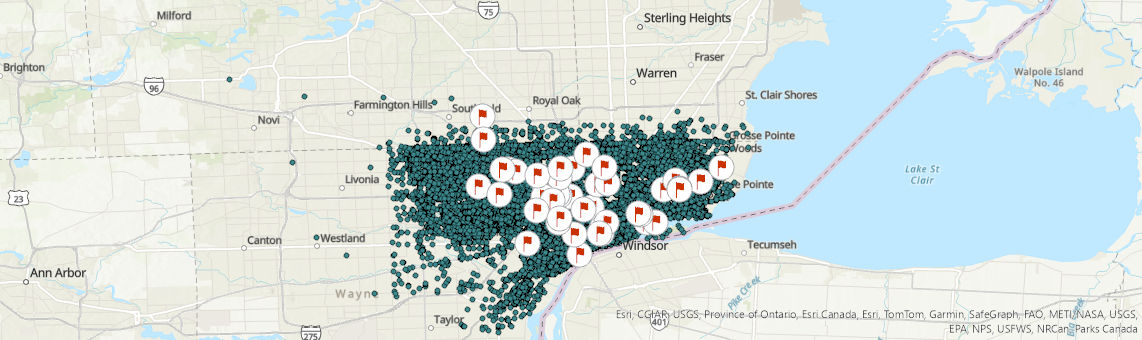
\includegraphics[width=0.75\linewidth]{Reproducibility Package/Visual Graphics/ArcGIS_Map.jpg}
    \caption{\textbf{911 calls and SATCs in Detroit Metro Area, 2017}}
    \label{fig:Figure2}
     \centering\small{Notes: This figure shows the distribution of the location of each 911 call and SATC in Detroit in 2017. The green dots are 911 calls, and the red flags in white circles are the locations of the substance abuse treatment centers. Although there are some outlying green dots in this figure, since we put a distance restriction of maximumn of 2,500 meters on the 911 calls counted, the outliers do not show up in any further dataset.}
    
\end{figure}

Figure~\ref{fig:Figure2} shows the plotted points from the data sets of all 911 calls and SATC from 2017. This is used to gather the data on each 911 call's distance to their closest SATC. This data allows each call to be sorted to its closest distance ring from each of the 44 SATCs. Although many points are close to multiple treatment centers, this allowed for each call to only be associated with a single SATC and to only be counted once. 



\subsection{Measuring Distance of each 911 Call to each SATC}
 


\begin{wrapfigure}[15]{r}{0.3\textwidth} 
 \begin{tikzpicture}
% Define the radii corresponding to the first 3 distances (in meters)

\centering
\def\radiusOne{0.5}
\def\radiusTwo{1}
\def\radiusThree{1.75}


% Draw the concentric circles
\foreach \r/\label in {\radiusOne/, 
    \radiusTwo/,
    \radiusThree/,}
 {
\draw[thick] (0,0) circle (\r);
    \node at (\r, 0) {\label};
    }   
    \fill (0,0) circle (2pt);
\end{tikzpicture}
\caption{\textbf{Concentric Distance Rings}}
\label{fig:Figure1}
\small{Notes: The figure represents the first three distance rings (250m, 500m, and 750m). Center dot marks the SATC.}
\end{wrapfigure}

We use layered data sets to map the 911 calls and SATC locations. We then create distance rings, referred to as distance groups, which are visualized in Figure~\ref{fig:Figure1}, to perform our analysis. After, we also normalize the data to account for differences in total area of a distance group that may alter results. We did this by dividing the total count of 911 calls in each distance ring by their respective areas in square meters. Then, we multiply by 1,000,000 to get the calls into count per kilometer squared.

We created concentric rings around each SATC. Each 911 point falls within one circle for a given treatment center.  The circles are referred to as a distance rings or distance groups. Each 911 point is counted towards the SATC in its circle's center. If the distance rings overlap each other, thereby overlapping the 911 calls it can be counted under, we count the data point only once and towards the SATC it is closer to. Our data is organized by SATC. We measured call points up to 2,500 meters away from a SATC. With this parameter, we analyze a total of 254,779 observations in 2017. We analyze the calls twice. First, we isolate and analyze 911 calls by 250-meter buckets. Then we conduct the same experiment, but with the observations organized by 500-meter concentric rings. This is to see if our resulting relationships are robust or not. The groups are named by the outer boundary of their ring. So, in the first data analysis, group 500-meter includes all calls from 250-500 meters from the SATC, while group 500 in the second part of data analysis would include all calls from 0-500 meters. We chose 250-meter intervals and 500-meter intervals since we wanted the distances to be of walking distance to a SATC, and for easy interpretation and comparison of the intervals. 
\begin{table}[H]
\centering
\scalebox{0.8}{
\centering
\begin{tabular}{l*{6}{c}}
\hline\hline
            &Summary\_Results&            &            &            &            &            \\
            &         Obs&        Mean&   Std. dev.&         Sum&         Min&         Max\\
\hline
250m        &          43&      1086.6&       821.4&     46721.8&           0&      4225.9\\
500m        &          43&         626&       419.1&     26919.7&           0&      1935.3\\
750m        &          43&       517.2&       374.7&     22240.9&           0&      1507.5\\
1000m       &          43&       392.1&       244.4&     16862.1&        34.9&      1185.2\\
1250m       &          43&       337.7&         253&     14522.3&           0&      1131.8\\
1500m       &          43&       211.1&       185.1&      9075.2&           0&       741.7\\
1750m       &          43&       165.8&       173.1&        7129&           0&       628.8\\
2000m       &          43&       123.2&       143.4&      5299.4&           0&       503.9\\
2250m       &          43&        98.2&       125.6&      4222.7&           0&       507.2\\
2500m       &          43&        65.1&        88.2&      2799.3&           0&       319.8\\
\hline\hline
\end{tabular}

}
\caption{\textbf{Summary Statistics of 2017 Calls in 250 Meter Intervals}}
\label{tabl:Table1}
\centering\small{Notes: In this table, we show the summary statistics of all 2017 Detroit 911 calls by distance group per substance abuse treatment center in the area. There are 10 distance groups, or "rings", ranging 250 meters apart from each other until 2500 meters in 250-meter intervals. Counts are normalized by the area of their rings, measured in kilometers squared. As the distance from SATC increases, the mean of 911 calls received decreases. Additionally, standard deviation decreases on average as the distance rings numerically increase. The most amount of calls seem to be in distances rings 750m, 1000m, and 1250m. Mean calls are standardized by dividing the total count of calls by their ring's area times 1,000,000. 1,000,000 was chosen to get mean calls into kilometers squared.}
\end{table}  

Table~\ref{tabl:Table1} includes the mean, standard deviation, total calls, and minimums and maximums of the total 2017 911 calls by 250-meter distances. By count, most of the calls happen in rings 750m-1250m, but on average, there tends to be more 911 calls closer to SATCs. For example, in the 500-meter groups, there are mean of 626 calls while the 1500-meter group has a mean of 211 calls. This trend could indicate that there are more calls located near SATCs as opposed to farther away. 

\begin{table}[hb!]
\centering
\scalebox{0.8}{
\centering
\begin{tabular}{l*{6}{c}}
\hline\hline
            &Summary\_Results\_2&            &            &            &            &            \\
            &         Obs&        Mean&   Std. dev.&         Sum&         Min&         Max\\
\hline
500m        &          43&    930.2742&    547.0896&    40001.79&           0&    2320.691\\
1000m       &          43&    761.5918&    440.2911&    32748.45&    130.2342&    2119.398\\
1500m       &          43&    487.3735&    375.6192&    20957.06&           0&    1623.728\\
2000m       &          43&    266.9263&    281.7036&    11477.83&           0&    1039.303\\
2500m       &          43&    152.9633&    196.6004&    6577.421&           0&    771.7172\\
\hline\hline
\end{tabular}

}
\caption{\textbf{Summary Statistics of 2017 Calls in 500 Meter Intervals}}
\label{tabl:Table2}
\centering\small{Notes: In this table, we show the summary statistics of all 2017 Detroit 911 calls by distance group per substance abuse treatment center in the area. There are 4 distance groups, or "rings", ranging 500 meters apart from each other to 2500 meters in 500-meter intervals. Counts are normalized by the area of their rings, measured in kilometers squared. The most amount of 911 calls are within the 500-meter ring. As the distance from SATC increases, the mean and total 911 calls received decreases. Additionally, standard deviation decreases on average as the distance rings numerically increase. The total amount of calls are in the 500m rings, at 40,001, and decreases as distance from SATC increases. Mean calls are standardized by dividing the total count of calls by their ring's area times 1,000,000. 1,000,000 was chosen to get mean calls into kilometers squared. }
\end{table}

Table~\ref{tabl:Table2} includes the mean, standard deviation, total calls, and minimums and maximums of the total 2017 911 calls by 500-meter distances. As the total 911 calls increases, the closer those calls are to an SATC become. For example, in the 500-meter groups, there are a mean of 930 calls, per kilometer squared the 1500-meter group has a mean of 487 calls. This trend also supports that there are more calls located near SATCs as opposed to farther away. 

%Describe your data. Where you got it from, how it was generated, what variables you'll use, what data cleaning steps you had to take, where your processed data, code and documentation is stored.
%In a published paper, a lot of this detail will be in a data appendix. For the purposes of this report, include it all here (this may be the longest section of your report).


\section{Results}
\label{sec:result}

This paper hypothesizes that as the distance from a SATC facility increases, the number of 911 calls also increases. This means that the farther someone is from a SATC, the less access they have to treat drug addiction, so the more likely they would exhibit drug-induced behavior that results in someone calling 911. Our null hypothesis is that there is no relation between distance to an SATC and the likelihood of calling 911.
\begin{table}[htbp]
\centering
\begin{tabular}{l|c c c c}
\hline
Comparison & Mean 1 & Mean 2 & Difference & P-value \\
\hline
250m-500m & 1086.6 & 626.0 & 460.5 & 0.000 \\
500m-750m & 626.0 & 517.2 & 108.8 & 0.071 \\
750m-1000m & 517.2 & 392.1 & 125.1 & 0.019 \\
1000m-1250m & 392.1 & 337.7 & 54.4 & 0.011 \\
1250m-1500m & 337.7 & 211.1 & 126.7 & 0.000 \\
1500m-1750m & 211.1 & 165.8 & 45.3 & 0.002 \\
1750m-2000m & 165.8 & 123.2 & 42.5 & 0.005 \\
2000m-2250m & 123.2 & 98.2 & 25.0 & 0.007 \\
\hline
\end{tabular}
\caption{\textbf{One-sample T-test Results by 250m Distance Rings}}
\label{tab:ttests1}
\centering\textit{This table shows one sample t-test in the difference of mean all calls per SATC per distance group. We got the means for each group by first assigning every 911 call the distance bucket they fall in respective to the SATC they are geographically closest to. Afterward, we divide each ring by its concentric ring's area* 1,000,000. We multiplied by 1,000,000 to offset the amount of negative number spaces seen when we divide total calls by their large areas. This way, our total and mean calls per area are not in the negatives so they are easier to see in the table. }
\end{table}
 
We conduct two pairwise one-sample t-tests to examine the statistical likelihood that one distance ring has a greater mean number of calls per SATC than the next larger ring. We chose to do one-sample t-tests instead of two-sample tests due to the dependent nature of our spatial data analysis and the large sample size we have. The first set of one-sample t-tests comparisons are in Table~\ref{tab:ttests_250}. These one-sample t-tests examine the mean calls per SATC between each adjacent distance group for all 2017 calls. We test at a confidence interval of 95\%. The mean calls are normalized by the ring area. 

The results of the majority of one-sample t-tests in Table~\ref{tab:ttests_250} support the rejection of the null hypothesis for seven of the eight one-sample t-tests. Five of the paired t-tests exhibit a p-value less than 0.01, indicating strong statistical significance between these sequential distance rings. In addition, two of the tests result in p-values less than 0.05, while one test (500-750meters) presents a p-value greater than 0.05, but less than 0.10. Although less strong than the groups mentioned above, it this shows some statistical significance. 
\begin{table}[htbp]
\centering
\begin{tabular}{l|c c c c}
\hline
Comparison & Mean 1 & Mean 2 & Difference & P-value \\
\hline
500m-1000m & 930.3 & 761.6 & 168.7 & 0.035 \\
1000m-1500m & 761.6 & 487.4 & 274.2 & 0.000 \\
1500m-2000m & 487.4 & 266.9 & 220.4 & 0.000 \\
2000m-2500m & 266.9 & 153.0 & 114.0 & 0.000 \\
\hline
\end{tabular}
\caption{\textbf{One-sample T-test Results by 500 meter Distance Rings}}
\label{tab:ttests_500}
\centering\footnotesize{This table shows one sample t-test in the difference of mean all calls per SATC per distance group by 500 meter intervals.}
\end{table}

\label{tabl:Table4}

For one of the one-sample t-tests, we cannot reject the null hypothesis as the p-value falls within the 95\% confidence interval. The 500-750 meter ring exhibits the p-value of 0.071. This high p-values indicates there is little evidence that the mean values of these distance rings are statistically significant. These results could be due to smaller mean differences, as seen in the column "Difference" when compared to the difference values in the t-test before and after it. Smaller difference values might mean that the data doesn't vary enough to make a meaningful difference. Having larger data samples might smooth out this issue. However, the lack of significance found could be caused by the range of distance parameters chosen. A change of distance of 250 meters might not be enough of a geo-spatial distance to properly isolate and identify distance trends around the SATC. 

This is why we conduct a one-sample t-test on larger distance intervals, the 500-meter interval set. The one-sample t-test comparison table is seen in Table~\ref{tab:ttests_500}. 

The results of the t-tests in Table~\ref{tab:ttests_500} support the rejection of the null hypothesis for the four t-tests conducted and further support the results identified in Table~\ref{tab:ttests_250}. Three of the tests reveal p-values equal to or less than 0.01, and the first one has a p-value of less than 0.05. Thus, all the t-tests in the 500-meter rings support the rejection of the null hypothesis, indicating there is a relationship between the variables. 

Every p-value in Table~\ref{tab:ttests_500} is smaller than the p-value in Table~\ref{tab:ttests_250}. The first group of Table~\ref{tab:ttests_500} has a weaker significance compared to the latter groups in the table, but this pattern lines up with p-values seen in the 500m-750m and 750m-1000m groups of Table~\ref{tab:ttests_250}. The p-value of group 500m-1000m in table~\ref{tab:ttests_500} is 0.035, just half of the p-value of group 500m-750m in table~\ref{tab:ttests_500}. The overall stronger statistical evidence in the second t-test table could be due to having more observations within each group, enhancing differences in means. This increases the confidence in the significance meaning of a difference in average calls.

\begin{figure}[htbp]
    \centering
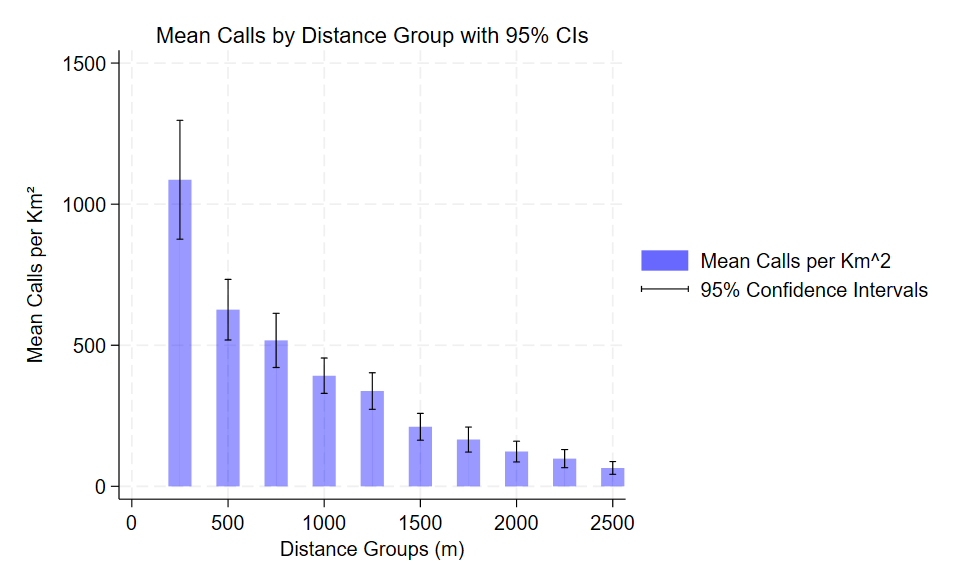
\includegraphics[width=0.75\linewidth]{Reproducibility Package/Downloaded_calls/Visual_Graphics_Downloaded_calls/250_CI_Graph.png}
    \caption{\textbf{Mean Calls per SATC per Distance Group}}
     \label{fig:Figure3}
     \centering\small{This figure shows mean calls per kilometer squared and 90\% confidence levels. The x-axis consists of the different distance groups used (100m, 250m, 500 m...2500m). Distance measured in meters.}
    \centering\small{Notes: The y-axis is measured in mean calls per kilometer squared. Each call was assigned one distance group for one SATC, so there is no double counting. The mean calls are counted to the upper bound of their ring.}
\end{figure}

Figure~\ref{fig:Figure3} represents the mean calls per SATC per kilometer squared by 250-meter distance groups in a bar graph. Figure~\ref{fig:Figure3} uses the same data as Table~\ref{tab:ttests_250}. Figure~\ref{fig:Figure4} represents the mean calls per SATC per square kilometer by 500-meter distance groups in a bar graph. Figure~\ref{fig:Figure4} uses the same data as Table~\ref{tab:ttests_500}. The confidence level of 95\% for mean calls is overlaid on top of their respective distance groups. 

In Figure~\ref{fig:Figure3}, the confidence intervals of 500 meters up until 2,500 meters significantly overlap. The significant overlap is due to the confidence interval of the farther distance group overlapping the mean and the confidence interval of the closer distance group. Since we conducted one-sample t-tests,  and the standard deviations seen in Table~\ref{tabl:Table1} are relatively close together, some overlap is to be expected. However, the large difference between 250 meters and 500 meters could further prove that, at least extremely close to SATCs, there is a significant increase in 911 calls. This indicates that there is some relationship between SATCs and the number of 911 calls extremely close to them, although the relationship may get hazier farther away from SATCs.

The other confidence intervals do have some overlap with the sequential intervals, but not as much. These confidence intervals in Figure~\ref{fig:Figure3} include 100-250 meters, 500-750 meters, 1000-1250 meters, 1250-1500 meters, 1500-1750 meters, 1750-2000 meters, 2000-2250 meters, and 2250-2750 meters. Due to the size of the graph, the last three confidence intervals are hard to visually identify, so looking at the p-values is crucial. 

\begin{figure}[H]
    \centering
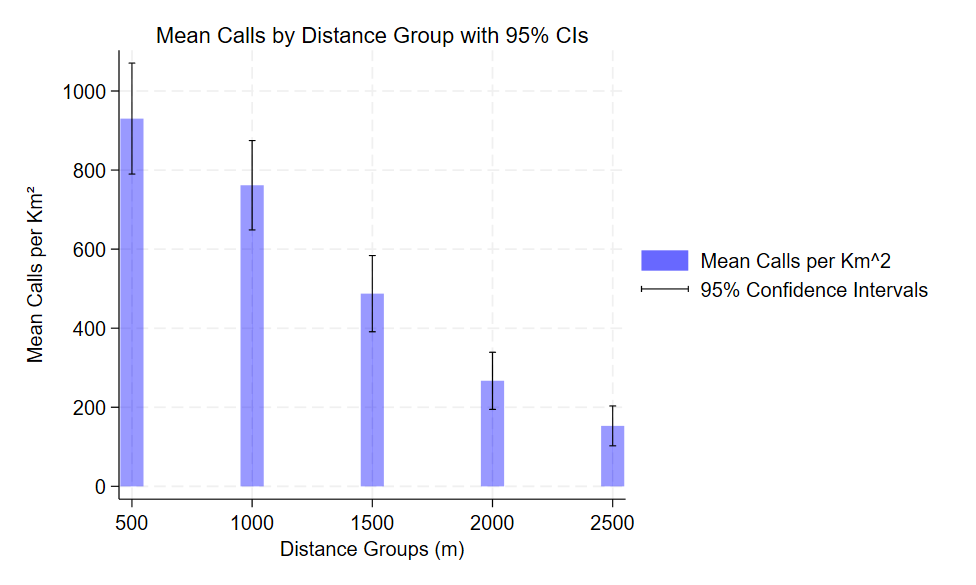
\includegraphics[width=0.75\linewidth]{Reproducibility Package/Downloaded_calls/Visual_Graphics_Downloaded_calls/500_CI_Graph.png}
    \caption{\textbf{Mean Calls per SATC per distance group}}
    \label{fig:Figure4}
       {This figure shows mean calls per kilometer squared and 90\% confidence levels. The x-axis consists of the different distance groups used (100m, 250m, 500 m...2500m). Distance measured in meters.}
    \centering\small{Notes: The y-axis is measured in mean calls per kilometer squared. Each call was assigned one distance group for one SATC, so there is no double counting. The calls are a smaller observation pool within total 2017 911 calls. The mean calls are counted to the upper bound of their ring.}
\end{figure}

Figure~\ref{fig:Figure4} also follows a similar, but less drastic, overlapping of confidence intervals. Since the means of the distance rings are more distance from each other. None of the confidence intervals in Figure~\ref{fig:Figure4} overlap with the means of adjacent distance groups. Since there are more observations for fewer groups, a more robust visual significance is to be expected. However, this figure further supports the strong negative correlation between 911 calls and proximity to SATCs. 


%Explain what analyses you did, provide evidence (like in the descriptive stats exercise, but refined and clear) and then explain what your results mean.
\break
\section{Discussion}
\label{sec:discussion}

One theory on why we find that as distance from a treatment center increases, the rate of 911 calls decreases is due to the feedback loop between drugs, crime, and lower standards of living in the area. SATCs are more likely to be built in areas where drug use is prevalent since higher levels of drug use are associated with a lower standard of living in an area. (\cite{drugs_and_crime}). This creates a feedback loop between increased drug use and lower living standards, leading to the establishment of SATCs. Moreover, \cite{drugs_and_crime} shows that lower standards of living are linked to higher crime rates and, consequently, reduced safety in an area. Therefore, areas with higher drug use lead to an increased likelihood of SATC being built there and a decrease in the standard of living in those areas. The decrease in the standard of living further reduces safety and increases crime. The lack of safety, in turn, leads to more 911 calls.  

Additionally, Detroit may have placed SATCs in neighborhoods with lower living standards due to pressure from more affluent communities. More affluent communities tend to exhibit a "Not In My Backyard" (NIMBY) mentality, opposing the placement of SATCs in their neighborhoods (\citealp{NIMBY}). This resistance stems from the fear or stigma residents have about drug users. They might perceive SATCs as bringing dangerous or mentally ill people into their area, impacting the safety of the area. Thus, higher standard-of-living neighborhoods tend to lobby for NIMBY policies in their communities, pushing SATCs to be in areas that do not have the resources to oppose their placement.

Furthermore, higher standard-of-living areas tend to have lower crime rates in general. High standards of living decreases crime, which creates a positive feedback system in these neighborhoods, potentially explaining why the farther a ring is from a SATC, the fewer 911 calls there are on average. Therefore, the distance rings that have fewer 911 calls on average could be on the cusp of, or geographically in neighborhoods that do not have SATCs. 
    
Another explanation for the lower frequency of 911 calls in further distance rings could be that we only consider each 911 call once in our analysis. When we geo-code the 911 calls, we assign each observation to only one SATC, the one geographically closest to it. The methodology behind this is to limit any overlap between 911 calls due to SATCs being geographically close together. Without this step, it could exaggerate the frequencies of 911 calls relative to an SATC and affect our measures in the smaller distance rings.  However, in farther distance rings, a call might be similar in distance to two SATCs but will only be assigned to one, when in reality, it could be assigned to either SATC. This could possibly lead to an underrepresentation of the frequency of 911 calls in the further distance rings. Therefore, this process of analysis could potentially be improved upon through finding a valid statistical test that would allow us to double count 911 calls, which could help resolve this issue. 

Moreover, one significant limitation was the inability to fine-tune 911 call data to determine whether calls were directly related to drug activity. Without additional data, such as toxicology reports or detailed incident descriptions, it remains challenging to assess the role of drugs in criminal behavior or whether the crimes involved were violent. A better understanding of what calls were drug-related or induced could provide more accurate results on the relationship between drug abuse, crime, and the role of a SATC in amplifying or mitigating crime in an area. 
    
Another limitation is the population density of this urban sample. The observed pattern of 911 calls can be influenced by higher population density in more highly populated neighborhoods in Detroit. A population in these areas naturally increases the number of emergency calls. However, specific information on the population density at the address level is not publicly available. Therefore, to precisely consider population density in relation to the number of 911 calls, we would need to geographically expand our area of analysis. However, expanding the geographical unit of analysis would not accurately allow us to study the effects an SATC has on the community immediately surrounding it. 

We analyzes data only from the year 2017. However, considering more years in our analysis would likely give us more statistical power. Therefore, we see future research supporting these findings or a stronger pattern through two possible ways. Firstly, by utilizing cross-sectional data for more than one year. The increase in data would likely strengthen the correlational relationships we found in this paper. Secondly, by analyzing time series data based on the openings and closings of SATCs. This option could identify a causal impact of the presence of a SATC in a neighborhood regarding 911 calls as a proxy for crime rates. These results could impact policymaking decisions regarding where to fund and support the placement of SATC to serve populations in need. 



\section{Conclusion}
\label{sec:conclusion}


We hypothesized that as the distance from a SATC increases, the frequency of 911 calls also increases. The closer a SATC is, the more accessible treatment is to a person whose behavior might be affected by drug abuse. Thus, closer treatment centers should reduce crime rates in the area, as measured by 911 calls. We conducted a cross-sectional analysis to examine how the distance from an SATC affects the frequency of 911 calls. Our results show that contrary to our hypothesis, as distance from a SATC increases, the amount of 911 calls per square kilometer decreases. This distance decay relationship indicates a relationship between SATC locations and 911 calls but in the opposite direction of the original hypothesis. We theorize that this could be due to the Not In My Backyard movement to prevent SATCs in areas with a higher standard of living or due to the feedback loop between drugs, crime, and lower standards of living. By better understanding the relationship between SATCs and crime rates, policymakers can better plan where SATCs should be placed to maximize welfare, in terms of boosting public safety and lowering drug abuse rates. 


 
%Re-state (in different words) what you did and what you learned. If your discussion (Section 6) would be short, you can just have a Conclusion section that includes your discussion (that is, leave out a separate Discussion section).

\newpage
\singlespacing
\setlength\bibsep{0pt}
\bibliography{WorkingFolder/sources.bib}
\bibliographystyle{chicago}



\newpage
\section*{Data Appendix} \label{sec:appendixa}
\addcontentsline{toc}{section}{Appendix A}

Our replication package:

\href{https://github.com/ecn310/course-project-zipcentercrime/tree/main/Reproducibility%20Package}{https://github.com/ecn310/course-project-zipcentercrime/tree/main/Reproducibility\%20Package}

\vspace{10pt}

% essentially, we should have a bunch of links to our files in the appendix section. 

We originally ran this project using the 911 call dataset Professor Deza gave us. She told us where to find the original off of the City of Detroit's Open Data Portal: \href{https://data.detroitmi.gov/datasets/detroitmi::police-serviced-911-calls/about}{Police Serviced 911 Calls}. This dataset did not match the dataset Professor Deza gave us completely. There were fewer observations in the 911 call dataset on the website than the dataset she provided us. In that dataset,there were 5,238,111 total observations, while the online dataset included 2,452,212. However, the variables and years were all the same. We ran the analysis with this new dataset, but besides there being fewer overall values, the statistical trends were the same. The confidence interval graphs followed the same trends, and the p-values seen from Table~ref/{Table}. We believe that the differences were due to the omission of specific call categories. Each 911 call gets assigned a category that it falls under, from assault and battery to traffic violations and check in class. We believe that most of the omitted calls were ones with non-criminal bearing. Additionally, the number of calls left was proportional to the amount of calls from before. The datasets, do files, and logs in this reproducibility project follow the dataset we accessed online. overall, our data analysis was robust under both datasets. the one sample t-tests and confidence intervals supported the same trends and significance levels. 

We also performed an analysis of only the crime-related calls. We used the variable call description to identify what calls could be considered to relate to crime. There are 466,219 observations in this subset. The purpose of this analysis is to focus on activities that drugs could cause. The 9-1-1 emergency telephone hotline is used for more than just crimes; it is used for any civil issue classified as an emergency. By focusing only on crime-related calls, we thought we could narrow down the issues to better estimate the impact of SATCs in an area. We theorized that if all calls to emergency services were considered, the results could be diluted by prioritizing areas with higher population densities. These people are not counted because they are unaffected by a SATC. Our analysis of this showed the same statistical patterns, so we conclude that the non-crime related calls don't dilute the where calls are being taken. 

The data files, code, and documentation for this project are found in the zipcentercrime \href{https://github.com/ecn310/course-project-zipcentercrime}{GitHub Repository}. All information and files necessary to reproduce these results can be accessed by this: \href{https://github.com/ecn310/course-project-zipcentercrime/tree/main/Reproducibility%20Package}{reproducibility package}. The code can be found in the \href{https://github.com/ecn310/course-project-zipcentercrime/tree/main/Reproducibility%20Package/Do%20files}{Do Files Folder}, and access the figures from this the \href{https://github.com/ecn310/course-project-zipcentercrime/tree/main/Reproducibility%20Package/Visual%20Graphics}{Visual Folder}. 

Use Stata 18.0 to isolate data to the year 2017 and for the final data analysis. Use ArcGIS Pro to geo-code the call points and SATC points. 

The original 911 calls dataset can be accessed from the \href{https://data.detroitmi.gov}{The City of Detroit Open Data Portal}. The raw dataset can be accessed from zipcentercrime repository at \href{https://github.com/ecn310/course-project-zipcentercrime/blob/main/Reproducibility%20Package/RawData/Acess_calls_final_data_set.md}{Acess\_calls\_final\_data\_set.md}. The original SATC dataset can be accessed from the \href{https://www.samhsa.gov}{SAMHSA website}. The raw dataset can be downloaded from the zipcentercrime repository through the \href{https://github.com/ecn310/course-project-zipcentercrime/blob/main/Reproducibility%20Package/RawData/detroit_samhsa_sud_2015_2021.dta}{detroit\_samhsa\_sud\_2015\_2021.dta file}.


\end{document}